\documentclass[landscape, 8pt]{extarticle}
\usepackage{geometry}
% \usepackage{showframe}
\usepackage[dvipsnames]{xcolor}

\colorlet{colour1}{Red}
\colorlet{colour2}{Green}
\colorlet{colour3}{Cerulean}

\geometry{
    a4paper, 
    margin=0.17in
}

\pretolerance=0
\hyphenpenalty=0

\usepackage{lmodern}

\usepackage[fontsize=7pt]{scrextend}

\usepackage{graphicx} % Required for inserting images
\usepackage{amsmath}
\usepackage{amsfonts}
\usepackage{amssymb}
% \usepackage{preamble}
\usepackage{enumitem}
\usepackage{multicol}
\usepackage{lipsum}
\usepackage[framemethod=TikZ]{mdframed}
% \usepackage{../thmboxes_white}
\usepackage{../thmboxes_v2}
\usepackage{float}
% \usepackage{setspace}
\usepackage[nodisplayskipstretch]{setspace}





% \setlength{\parskip}{0pt}

% Custom Definitions of operators
\DeclareMathOperator*{\argmax}{arg\,max}
\DeclareMathOperator*{\argmin}{arg\,min}
% \DeclareMathOperator{\im}{im}
% \DeclareMathOperator{\Fix}{Fix}
% \DeclareMathOperator{\Orb}{Orb}
% \DeclareMathOperator{\Stab}{Stab}
% \DeclareMathOperator{\send}{send}
% \DeclareMathOperator{\dom}{dom}
% \DeclareMathOperator{\Maps}{Maps}
% \DeclareMathOperator{\sgn}{sgn}
% \DeclareMathOperator{\Mat}{Mat}
% \DeclareMathOperator{\scale}{sc}
% \DeclareMathOperator{\Hom}{Hom}
% \DeclareMathOperator{\id}{id}
% \DeclareMathOperator{\rk}{rk}
% \DeclareMathOperator{\Tr}{tr}
% \DeclareMathOperator{\diag}{diag}
% \DeclareMathOperator{\can}{can}

\usepackage{hyperref} % note: this is the final package

\parindent = 0pt

\renewcommand\labelitemi{\tiny$\bullet$}

\begin{document}

\setlength{\abovedisplayskip}{3.5pt}
\setlength{\belowdisplayskip}{3.5pt}
\setlength{\abovedisplayshortskip}{3.5pt}
\setlength{\belowdisplayshortskip}{3.5pt}

\begin{multicols}{3}
\raggedcolumns


\section*{\huge FNLP Exam Notes}
Made by Leon :) 
\vspace{-5pt}
\section{smooth and stuff}

\begin{dfn}[Maximum Likelihood Estimates (MLE)]{dfn:mle}{}
    \[P_{RF}(x) = \frac{C(x)}{N}\]
    $C(x)$ is the count of $x$ in the dataset, and $N$ is the total number of items in the dataset

    \begin{itemize}[leftmargin=*]
        \setlength\itemsep{0em}
        \item \textbf{Problem 1 (Sparse data problem)}: If the count of an item is $0$, then the probability will also be $0$ - you want the model to be able to calculate sentences with new words in them. \textbf{Solution}: Smoothing
        \item \textbf{Problem 2}: Cannot reliably find probability of sentences (the chance of ``skibidi sigma gyatt rizz'' being already in a corpus is very low). \textbf{Solution}: use $n$-gram models
    \end{itemize}
\end{dfn}

\begin{dfn}[n-gram models]{dfn:ngrams}{}
    Turn a sentence $P(S = w_{1}\dots w_{n})$ into joint probabilities $P(w_{1},\dots,w_{n})$. We have $P(X, Y) = P(Y | X)P(X)$. So
    \begin{align*}
        P(a, b, c) &= P(c | a,b)P(a,b)\\
                            &= P(c | a, b)P(b|a)P(a)
    \end{align*}

    n-gram model just estimates probability to $n$ probabilities
    \begin{itemize}[leftmargin=*]
        \setlength\itemsep{0em}
        \item \textbf{Trigram}: $P(w_{i}|w_{1},w_{2},\dots,w_{i-1}) \approx P(w_{i}|w_{i-2}, w_{i-1})$
        \item \textbf{Bigram}: $P(w_{i}|w_{1},w_{2},\dots,w_{i-1}) \approx P(w_{i}|w_{i-1})$
        \item \textbf{Unigram}: $P(w_{i}|w_{1},w_{2},\dots,w_{i-1}) \approx P(w_{i})$
    \end{itemize}

    \noindent\rule{\textwidth}{0.2pt}
    To be able to detect edges of sentences, add \texttt{<s>} and \texttt{<\symbol{92}s>} on sentence edges to be factored into the $n$-gram model
    \[\text{\texttt{skibidi rizz}} \implies \text{\texttt{<s> skibidi rizz <\symbol{92}s>}}\]
    therefore a bigram like $P(\text{\texttt{<\symbol{92}s>}} | \tt{rizz})$ will detect the end of a sentence 

    Usually, \textbf{negative log probs} will be used instead of regular decimals, as the probabilities will get small fast and floating precision issues will happen.
    \begin{itemize}[leftmargin=*]
        \setlength\itemsep{0em}
        \item Probabilities from 0 to 1, but negative log probs go from 0 to $\infty$
        \item Log probs are added instead of multiplied like regular probabilities
    \end{itemize}
\end{dfn}

\begin{dfn}[Entropy]{dfn:entropy}{}
    \textbf{Entropy} of a random variable $X$:
    \[H(X) = \sum_{x} - P(x) \log_{2}P(x)\]
    also the expected value of $-\log_{2}P(X)$

    Higher entropy means less predictable

    \begin{figure}[H]
        \centering
        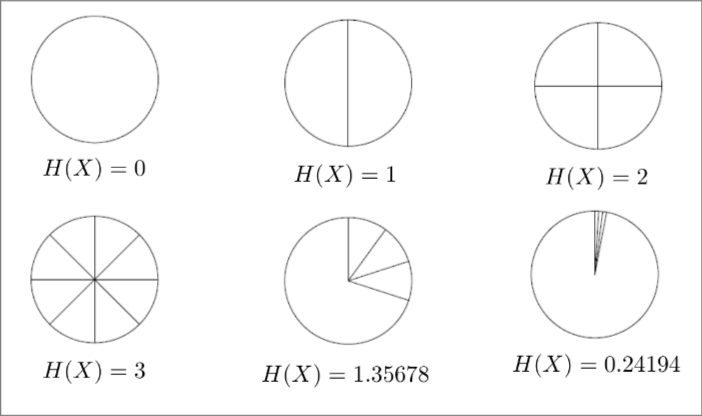
\includegraphics[width=0.6\linewidth]{images/2024-05-09-111807_hyprshot.png}
    \end{figure}

    For $w_{1}\dots w_{n}$ with large $n$, per-word cross-entropy is well approximated by
    \[H_{M}(w_{1}\dots w_{n}) = -\frac{1}{n} \log_{2}P_{M}(w_{1}\dots w_{n})\]
    Lower cross-entropy $\implies$ model is better at predicting next word

    \textbf{Perplexity}: $2^{\text{cross-entropy}}$
\end{dfn}


\begin{dfn}[Add-one and Lidstone smoothing]{dfn:add-one-lidstone-smoothing}{}
    \textbf{Add one smoothing}
    \[P_{+1}(w_{i} | w_{i-2}, w_{i-1}) = \frac{C(w_{i-2}, w_{i-1}, w_{i}) + 1}{C(w_{i - 2}, w_{i-1}) + v}\]
    where $v$ is the vocabulary size

    \noindent\rule{\textwidth}{0.2pt}

    \textbf{Add-$\alpha$ smoothing}
    \[P_{+\alpha}(w_{i} | w_{i - 1}) = \frac{C(w_{i-1}, w+i) + \alpha}{C(w_{i-1}) + \alpha v}\]

    Choosing an $\alpha$: Use a three-way data split: \textbf{training set} (80-90\%), \textbf{held-out/development set} (5-10\%), and \textbf{test set} (5-10\%)
    \begin{itemize}
        \setlength\itemsep{0em}
        \item Train model (estimate probabilities) on training set with different values of $\alpha$
        \item Choose the $\alpha$ that minimizes cross-entropy on development set
        \item Report final results on test set
    \end{itemize}
    More generally, use development set for evaluating different models, debugging, and optimizing choises. This avoids overfitting to the training set and even to the test set

\end{dfn}

\begin{dfn}[Good-Turing Smoothing]{dfn:good-turing}{}
    \[c* = (c + 1) \frac{N_{c+1}}{N+c} \qquad P*_{c} = \frac{c*}{N} = (c + 1) \frac{\frac{N_{c+1}}{N_{c}}}{N}\]

    \begin{itemize}[leftmargin=*]
        \setlength\itemsep{0em}
        \item $N_{c}$ is the number of occurances with count $c$
        \item $P*_{c}$ is the probability of an item with count $c$
        \item $c*$ is the good-turing smoothed version of count
        \item $N$ is total count
    \end{itemize}

    \textbf{random items}
    \begin{itemize}
        \setlength\itemsep{0em}
        \item Probability the next observation is new
            \[P(unseen) = \frac{N_{1}}{N}\]
        \item Probability the next observation is a specific new object
            \[P_{GT} = \frac{1}{N_{0}} \frac{N_{1}}{N} \implies c* = \frac{N_{1}}{N_{0}}\]
    \end{itemize}

    \noindent\rule{\textwidth}{0.2pt}
    \textbf{Problems with Good-Turing}
    \begin{itemize}
        \setlength\itemsep{0em}
        \item Assumes we know the vocabulary size
        \item Doesn't allow "holes" in the counts (if $N_{i}>0,N_{i-1}>0$)
        \item Applies discounts even to high-frequency items
        \item Assigns equal probability to all unseen events, same with add-$\alpha$, e.g. ``w rizz'' vs ``w indowpane'' shouldn't be equal
    \end{itemize}
\end{dfn}

\begin{dfn}[Interpolation and backoff]{dfn:interpolation-backoff}{}
    \textbf{Interpolation}: Combines higher and lower order $N$-gram models, since they have different strengths and weaknesses
    \begin{itemize}[leftmargin=*]
        \setlength\itemsep{0em}
        \item high-order $N$-grams are sensitive to more context, but have sparse counts
        \item low-order $N$-grams have limited context but robust counts
    \end{itemize}

    If $P_{N}$ is $N$-gram estimate
    \[P_{\text{INT}}(w_{3}|w_{1},w_{2}) = \lambda_{1}P_{1}(w_{3}) + \lambda_{2}P_{2}(w_{3}|w_{2}) + \lambda_{3}P_{3}(w_{3}|w_{1},w_{2})\]

    \textbf{Katz-backoff}: Trust the highest order language model that contains the $N$-gram. Requires an adjusted prediction model: $P*(w_{i}|w_{i-N+1},\dots,w_{i-1})$ and backoff weights: $\alpha(w_{1},\dots,w_{N-1})$
        
    \textbf{Kneser-Ney}: Takes diversities of histories into account
    \begin{itemize}
        \setlength\itemsep{0em}
        \item count of distinct histories for a word
            \[N_{1+}(\circ w_{i}) = \lvert \{w_{i-1} : c(w_{i-1}, w_{i}) > 0\} \rvert\]
        \item In $KN$ smoothing, replace raw counts with count of histories:
            \[P_{\text{ML}}(w_{i}) = \frac{C(w_{i})}{\sum_{w}C(w)} \quad \implies P_{\text{KN}}(w_{i}) = \frac{N_{1+(\circ w_{i})}}{\sum_{w} N_{1+}(\circ w)}\]
    \end{itemize}

    \noindent\rule{\textwidth}{0.2pt}
    Method use cases:
    \begin{itemize}
        \item Uniform probabilities - add-$\alpha$, Good-Turing
        \item Probabilities from lower-order $n$-grams - interpolation, backoff
        \item Probability of appearing in new contexts - Kneser-Ney
    \end{itemize}
\end{dfn}

\newpage
\section{Text Classification}
\vspace{-5pt}
Categorizing the \textit{content} of the text. e.g.
\vspace{-2pt}
\begin{itemize}
    \setlength\itemsep{0em}
    \item Spam detection (binary classification: spam/not spam)
    \item Sentiment analysis (binary / multiway)
        \vspace{-2pt}
        \begin{itemize}
            \setlength\itemsep{0em}
            \item movie, restaurant, product reviews (pos/neg, or 1-5 stars)
            \item political argument (pro/con or pro/con/neutral)
        \end{itemize}
    \item Topic classification (multiway: sport/finance/travel/etc)
\end{itemize}
Or, categorizing the \textit{author} of the text (authorship attribution)
\vspace{-2pt}
\begin{itemize}
    \setlength\itemsep{0em}
    \item Native language identification (e.g. to tailor language tutoring)
    \item Diagnosis of disease (psychiatric or cognitive impairments)
    \item Identification of gender/dialect/educational background (e.g. forensics [legal matters], advertising/marketing)
\end{itemize}

$n$-gram models are not as useful for classification - often we can just consider a \textbf{bag of words} and not worry about the order that the words come in

\begin{dfn}[Naive Bayes]{dfn:naive-bayes}{}
    \vspace{-5pt}
    Given document $d$ and set of categories $C$ we want to assign $d$ to the most probable category $\hat{c}$
    \[\hat{c} = \argmax_{c\in C} P(c | d) = \argmax_{c\in C} P(d|c)P(c)\]

    Represent $d$ as the set of features (words) it contains: $f_{1},f_{2},\dots,f_{n}$
    \[P(d | c) = P(f_{1},f_{2},\dots,f_{n} | c)\]
    Then make \textbf{naive Bayes assumption} that features are conditionally independent given the class
    \[P(f_{1},f_{2},\dots,f_{n}|c) \approx P(f_{1}|c) P(f_{2}|c)\dots P(f_{n}|c)\]
    i.e. the probability of a word happening depends \textbf{only} on the class, not on words occuring before/after (n-gram), or even what other words occurred at all. Basically we only care about the \textbf{count} of each feature in a document

    \vspace{-5pt}
    \noindent\rule{\textwidth}{0.2pt}
    \textbf{Naive Bayes classifier}: Given a document with features $f_{1},f_{2},\dots,f_{n}$ and set of categories $C$, choose the class $\hat{c}$ where
    \[\hat{c} = \argmax_{c\in C} P(c)\prod_{i=1}^{n}P(f_{i}|c)\]
    \begin{itemize}[leftmargin=*]
        \setlength\itemsep{0em}
        \item $P(c)$ is the \textbf{prior probability} of class $c$ before observing any data. normally estimated with MLE:
            \[\hat{P}(c) = \frac{N_{c}}{N}\]
            \begin{itemize}
                \setlength\itemsep{0em}
                \item $N_{c}$ is the number of training documents in class $c$
                \item $N$ is the total number of training documents. 
            \end{itemize}
            \vspace{-5pt}
            Therefore, $\hat{P}(c)$ is the proportion of training documents in class $c$
        \item $P(f_{i}|c)$ is the probability of seeing feature $f_{i}$ in class $c$. Normall estimated with simple smoothing:
            \[\hat{P}(f_{i}|c) = \frac{\text{count}(f_{i}, c) + \alpha}{\sum_{f\in F}(\text{count}(f, c) + \alpha)}\]
            \begin{itemize}
                \setlength\itemsep{0em}
                \item $\text{count}(f_{i}, c)$: the number of times $f_{i}$ occurs in class $c$
                \item $F$: the set of possible features
                \item $\alpha$: the smoothing parameter, optimized on held-out data
            \end{itemize}

    \end{itemize}

    \vspace{-10pt}
    \noindent\rule{\textwidth}{0.2pt}
    Same with $n$-gram models, usually uses \textbf{negative log probabilities} - adjusted equation:
    \[\hat{c} = \argmin_{c\in C} + (-\log P(x) + \sum_{i = 1}^{n} -\log P(f_{i} | c))\]
    This amounts to classification using a linear function (in log space) of the input features. Therefore Naive bayes is called a \textbf{linear classifier}
\end{dfn}

\columnbreak

\textbf{Issues with choosing features}
\begin{itemize}
    \setlength\itemsep{0em}
    \item Sentiment analysis might need domain-specific non-sentiment words e.g. ``quiet'' or ``memory'' for computer reviews
    \item Stopwords might be useful features for other tasks, e.g. People with schizophrenia use more 2nd-person pronouns, and people with depression use more 1st-person
    \item Probably better to use too many irrelevant feaetures than not enough relevant ones
\end{itemize}

\textbf{Problems with annotation}: Usually hard to come by already annotated text - ergo you need someone to label text. On the other hand there is usually a lot of unannotated texts.

\textbf{Solution}: Use semi-supervised learning
\begin{enumerate}
    \setlength\itemsep{0em}
    \item Train NB on labeled data alone
    \item Predict labels on unlabelled data
    \item Re-estimate NB, but now using also self-labelled data
\end{enumerate}

\textbf{Self Training}
\begin{itemize}
    \setlength\itemsep{0em}
    \item \textbf{Advantages}: Simplicity and applicable to any classifier
    \item \textbf{Disadvantages}: Does not account for uncertainty of a classifier, and no theoretical motivation
    \item To make it work needs discarding low-confidence predictions, and curriculum (start with examples similar to labeled data)
\end{itemize}

\textbf{Expectation Maximisation for Semi-supervised Learning}

\begin{itemize}
    \setlength\itemsep{0em}
    \item Train NB on labelled data alone
    \item Make soft prediction on unlabelled data (``E-step'')
    \item Recompute NB parameters using the soft counts
\end{itemize}

Self-training for NB is known as ``hard EM''

\textbf{Advantages of Naive Bayes}
\begin{itemize}
    \setlength\itemsep{0em}
    \item Very easy to implement
    \item Very fast to train and classify new docs (good for huge datasets)
    \item Doesn't require as much training data as some other methods (good for small datasets)
    \item Usually works reasonably well
    \item Should be the baseline method for any classification task
\end{itemize}

\textbf{Evolving past naive Bayes}: 
\begin{itemize}
    \setlength\itemsep{0em}
    \item Assuming that all features are conditionally independent can have some issues, and often we have enough training data for a better model.
    \item Adding multiple feature types (e.g. words and morphemes) often leads to even stronger correlations between features
    \item Accuracy of classifier can sometimes still be ok, but it will be highly overconfident in its decision, e.g. NB sees 5 features that all point to class 1, treats them as 5 independent sources of evidence - like asking 5 friends for an opinion when some got theirs from each other
\end{itemize}

\begin{dfn}[Maximum Entropy / Logistic Regression]{dfn:maxent-logreg}{}
    Most commonly \textbf{multinomial logistic regression}. \textbf{multinomial} if more than two possible classes, otherwise just \textbf{logistic regression}

    Like Naive Bayes, assign a document $x$ to class $\hat{c}$ where
    \[\hat{c} = \argmax_{c\in C} P(c |x)\]
    unlike Naive Bayes, model $P(c|x)$ directly instead of using Baye's rule

    \noindent\rule{\textwidth}{0.2pt}

    \textbf{Discrimination}
    \begin{itemize}
        \item Trained to discriminate correct vs wrong values of $c$ given input $x$
        \item Need not be probabilistic
        \item Examples: artificial neural networks, decision trees, nearest neighbour methods, support vector machines
        \item Here we only consider one method: MaxEnt models which are probabilistic
    \end{itemize}

    \noindent\rule{\textwidth}{0.2pt}
    \textbf{Feature Functions}: Like Naive Bayes, MaxEnt models use \textbf{features} we think will be useful for classification.

    However, features are treated different in the two models
    \begin{itemize}
        \setlength\itemsep{0em}
        \item NB: Features are \textbf{directly observed} (e.g. words in doc): no difference between features and data
        \item MaxEnt: We will use $\vec{x}$ to represent the observed data. Features are \textbf{functions} that depend on both observations $\vec{x}$ and class $c$
    \end{itemize}

    \noindent\rule{\textwidth}{0.2pt}
    \textbf{Classification with MaxEnt}
    
    Choose the class that has highest probability according to
    \[P(c | \vec{x}) = \frac{1}{Z} \exp\left(\sum_{i}w_{i}f_{i}(\vec{x}, c)\right)\]
    \begin{itemize}
        \setlength\itemsep{0em}
        \item Normalization constant $Z = \sum_{c'}\exp(\sum_{i}w_{i}f_{i}(\vec{x},c))$
        \item Inside brackets is just a dot product $\vec{w} \cdot \vec{f}$
        \item $P(c|\vec{x})$ is a \textbf{monotonic function} of this dot product
        \item So, we will end up choosing the class for which $\vec{w} \cdot \vec{f}$ is highest
    \end{itemize}

    \noindent\rule{\textwidth}{0.2pt}
    \textbf{Training the model}
    Given annotated data, choose weights that make the labels most probable under the model
    That is, given items $x^{(1)}\dots x^{(N)}$ with labels $c^{(1)}\dots c^{(N)}$, choose
    \[\hat{w} = \argmax_{\vec{w}} \sum_{j} \log P(c^{(j)} | x^{(j)})\]
    This is called \textbf{conditional maximum likelihood estimation} (CMLE)

    Like MLE, CMLE will overfit, so use \textbf{regularization} to avoid that

\end{dfn}


\textbf{Relation to Naive Bayes} - Naive Bayes is also a linear classifier, and can be expressed in the same form. Should the features actually be independent they would converge to the same solution as the amount of training data increases

\textbf{Downside to MaxEnt models}
\begin{itemize}
    \setlength\itemsep{0em}
    \item Supervised MLE in generative models is easy - compute counts and normalize
    \item Supervised CMLE in MaxEnt is not so easy
        \begin{itemize}
            \setlength\itemsep{0em}
            \item requires multiple iterations over the data to gradually improve weights (using gradient ascent)
            \item Each iteration computese $P(c^{(j)} | x^{(j)})$ for all $j$, and each possible $c^{(j)}$
            \item This can be time-consuming, especially if there are a large number of classes and/or thousands of features to extract from each training example
        \end{itemize}
\end{itemize}

\textbf{Robustness: MaxEnt and Naive Bayes}
\begin{itemize}
    \setlength\itemsep{0em}
    \item Imagine that in training there is one very frequent predictive feature, e.g. in training sentiment data contained emoticons but not at test time
    \item The model can quickly learn to rely on this feature
        \begin{itemize}
            \setlength\itemsep{0em}
            \item model is confident on examples with emoticons
            \item the gradient on these examples gets close to zero
            \item the model does not learn other features
        \end{itemize}
    \item In MAxEnt, a feature weight will depend on the precense of other predictive features
    \item Naive Bayes will rely on all features - the weight of a feature is not affected by how predictive other features are
    \item This makes NB more robust than (basic) MaxEnt when test data is (distributionally) different from training data
\end{itemize}

\lipsum[1-12]
\end{multicols}
\end{document}
